\documentclass[11pt]{article}
\usepackage{times}
\usepackage{geometry}
\geometry{letterpaper, portrait, margin=1in}
\usepackage[utf8]{inputenc}
\usepackage{enumitem,amssymb}
\usepackage{ragged2e}
\usepackage{graphicx}
\usepackage{comment}
\usepackage{multicol}
\usepackage[usenames]{xcolor} %used for font color              
\definecolor{xlinkcolor}{cmyk}{1,1,0,0}
\usepackage{url}
\usepackage[
 colorlinks=true,    % false: boxed links; true: colored links 
 linkcolor=xlinkcolor,     % color of internal links            
 citecolor=xlinkcolor,     % color of links to bibliography
 filecolor=xlinkcolor,  % color of file links 
 urlcolor=xlinkcolor,      % color of external link
 final=true
]{hyperref}
\usepackage[super,sort&compress]{natbib}
\usepackage{enumitem}
\setenumerate{itemsep=0mm}
\usepackage{xspace}

\setlength{\parskip}{0.5em}

\bibliographystyle{naturemag-doi}

\newcommand{\RST}{\emph{Roman}\xspace}

\begin{document}
\begin{raggedright} 
% part of template, but does not look good
\huge
Snowmass2021 - Letter of Interest \hfill \\[+1em]
\textit{Roman Space Telescope Strong Lensing Probes of Dark Matter Substructure} \hfill \\[+1em]
\end{raggedright}

\normalsize

\noindent {\large \bf Thematic Areas:}  (check all that apply $\square$/$\blacksquare$)

\noindent $\square$ (CF1) Dark Matter: Particle Like \\
\noindent $\square$ (CF2) Dark Matter: Wavelike  \\ 
\noindent $\blacksquare$ (CF3) Dark Matter: Cosmic Probes  \\
\noindent $\square$ (CF4) Dark Energy and Cosmic Acceleration: The Modern Universe \\
\noindent $\square$ (CF5) Dark Energy and Cosmic Acceleration: Cosmic Dawn and Before \\
\noindent $\square$ (CF6) Dark Energy and Cosmic Acceleration: Complementarity of Probes and New Facilities \\
\noindent $\square$ (CF7) Cosmic Probes of Fundamental Physics \\
\noindent $\square$ (Other) {\it [Please specify frontier/topical group]} \\

\noindent {\large \bf Contact Information:} (authors listed after the text)\\
Submitter Name/Institution: Brant Robertson (University of California, Santa Cruz\\
Collaboration: Nancy Grace Roman Formulation Science Working Group\\
Contact Email: brant@ucsc.edu\\

\noindent {\large \bf Abstract:}
\emph{Nancy Grace Roman Space Telescope}, formerly known as 
the \emph{Wide Field Infrared Survey Telescope}, is scheduled to launch in the mid-2020's and will provide a
multi-band, high-resolution view of the cosmos. Equipped with a mirror the size of \emph{Hubble
Space Telescope} and a $0.3~\mathrm{deg}^2$ infrared-sensitive camera $\sim100\times$ larger than \emph{Hubble/Wide Field Camera 3},
\RST will efficiently and sensitively map large areas of the sky with $\sim0.1''$ resolution.
This resolution will enable the discovery of $\sim 1000$ gravitationally-lensed quasars, which 
in turn provide detailed constraints on the properties of dark matter substructures. We
review the promise of \RST for achieving dark matter constraints through strong lensing,
both as stand-alone lensing experiment and in collaboration with other facilities.

\clearpage

% LOI text
\noindent %{\it Insert your white paper text here (maximum of 2 pages including figures).}

\emph{Nancy Grace Roman Space Telescope} (\RST) is a 2.4m space telescope scheduled 
to be launched in the
mid-2020's by the United States National Aeronautics and Space Administration (NASA)\citep{spergel2015a,akeson2019a}.
Formerly known as the \emph{Wide Field Infrared Survey Telescope}, \RST will undertake
an ambitious set of mission surveys including a large area cosmology survey ($\sim 2000~\mathrm{deg}^2$)
with multiband imaging ($H\sim26.7$AB flux limit) and slitless grism spectroscopy ($\sim10^{-16}~\mathrm{erg}~\mathrm{s}^{-1}~\mathrm{cm}^{-2}$ line sensitivity at $\lambda\sim1.5\mu$m).

While the cosmology mission surveys are designed to constrain structure formation and the
expansion history through weak lensing and baryon acoustic oscillations, 
\RST can test our picture for small-scale dark matter structure formation more
directly through gravitational lensing. The cold dark matter plus cosmological constant ($\Lambda$CDM)
paradigm forms one of the pillars of our models for the origin and evolution of cosmic structures.
While remarkably successful at matching observations on large scales, there have been persistent
observational challenges to the cold, collisionless dark matter expectations on dwarf-galaxy
scales. These “small-scale controversies” may simply stem from a poor understanding of the
baryonic processes involved in galaxy formation, or indicate more complex dark sector physics\citep{bullock2017a}.

Detailed testing of the standard paradigm on small scales remains one of the most pressing issues
in cosmology. Numerical simulations in $\Lambda$CDM predict a rich spectrum of substructure in galaxy
halos. Small fluctuations in the galaxy-scale lensing potential caused by these substructures
should result in measurable “flux anomalies” in the magnifications of quadruply-lensed quasar
images \citep{metcalf2001a}. While discrepancies between the observed flux ratios and
those predicted by a smooth lens model may have been found in quasar lenses \citep{mao1998a,dalal2002a,metcalf2002a}, the small size of current samples limits our understanding ($\sim56$
quad lenses\citep{lemon2020a}, even fewer with high-resolution imaging). According to predictions of the
occurrence of multiply-imaged strong-lensed quasars in wide-area surveys\citep{oguri2010a},
the \RST cosmology
survey will revolutionize this field
by increasing the sample of quad lenses by more than 20$\times$ to $\sim1000$ objects.



The ability to use strong-lensed quasars as probes of the small-scale structure of dark matter halos
can be powerful for constraining the nature of dark matter itself. The quasar strong-lensing method is
potentially sensitive to the presence of any
dark matter component that may suppress small-scale power. Subhalos in the host galaxy lens and
in structures along the line of sight\citep{hsueh2020a} affect the image positions and flux ratios. By
modeling how the mass function of subhalos, which is directly controlled by the small-scale
power spectrum, influences the lensing signal, the presence of a warm dark matter component can
be constrained. For instance, \cite[Gilman et al. 2020][]{gilman2020a} used space-based imaging\citep{nierenberg2020a}
of only 8 multiply-lensed quasars to place 95\% confidence limits of $m_{DM}>5.2$ keV assuming thermal relics.
With increased samples of dozens of quad-image strong lenses with high-resolution imaging, constraints can be
achieved\citep{despali2020a} on sterile neutrino dark matter models with masses $m_{DM}\sim7$keV required to explain the 3.5keV line seen in \emph{XMM-Newton} and \emph{Chandra} x-ray
data\citep{bulbul2014a,boyarsky2015a,cappelluti2018a}.

Over the last decade, methods have been developed to use extended lensed sources, in addition to the
point-like AGN, to identify substructures through distortions of lensed images. Extended sources
are imaged into arcs and rings that probe a larger volume in the lens halo, increasing the number
of subhalos that can be sensed. They also can be drawn from larger populations of background
sources, typical galaxies rather than bright AGN. \cite[Vegetti \& Koopman (2009)][]{vegetti2009a} described a
method for identifying substructures with high-resolution optical/IR imaging of extended
galaxies, with \cite[Vegetti et al. (2012)][]{vegetti2012a} reporting a detection of a dark substructure in a gravitational
lens at $z=0.9$. 
In related work, \cite[Hezaveh et al. (2013, 2016a)][]{hezaveh2013a,hezaveh2016a} described the use of (sub-)millimeter
spectral lines from dusty lensed galaxies to search for subhalos in the lenses. The wide survey
area of the \RST cosmology survey, along with its combination of multi-band imaging and spectroscopy, will provide
many avenues for identifying large samples of lensed galaxies for such substructure searches.
By combining space-based and ground-based surveys\citep{agnello2018a,anguita2018a,everett2020a}, 
\RST can contribute by extending strong-lensing probes of dark matter to halo inner density
profile slope measurements\citep{gavazzi2007a,fiacconi2016a,wong2017a}, group-to-cluster scale lenses\citep{jaelani2020a},
and statistical measures of the matter power spectrum\citep{diaz_rivero2018a}.


\begin{figure}
\begin{center}
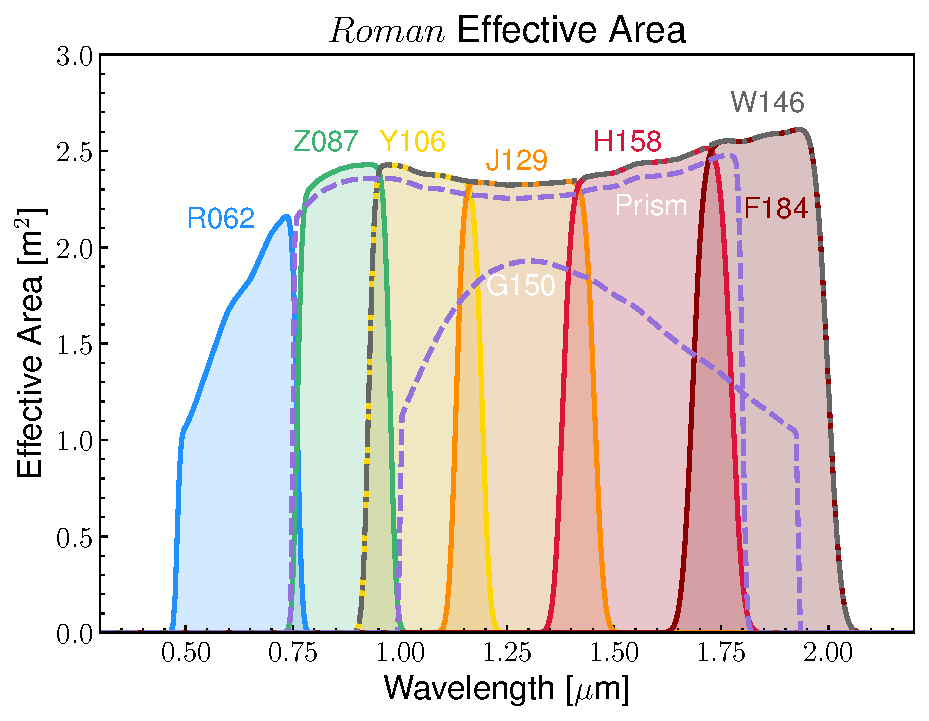
\includegraphics[width=0.47\textwidth]{roman_effective_area_color.pdf}
\end{center}
\caption{Effective area of \RST in its multiband photometric and grism spectroscopic bands as a function of wavelength (updated from \citep[Akeson et al. 2019][]{akeson2019a}). Shown are the $R062$ (blue), $Z087$ (green), $Y106$ (yellow), $J129$ (orange), $H158$ (red), $F184$ (crimson), and $W146$ (gray dot-dashed) photometric filters, and the G150 and Prism spectroscopic filters (purple dashed). The high-resolution multiband imaging and slitless spectroscopy will enable \RST to constrain substructure in individual lenses and thereby provide information on the nature of dark matter.}
\label{fig:effective_area}
\end{figure}

While \RST covers smaller areas than either \emph{Euclid} from space or \emph{Vera Rubin Observatory} from the ground, the potency of \RST to provide improved constraints on the small-scale matter power spectrum
through lensing is significantly enhanced by its high-resolution, ultradeep, space-based, multiband imaging
and grism spectroscopy. The \RST cosmology survey is expected to have $Y$, $J$, and $H$ filter
images, along with additional coverage in the $F184$ filter that extends to $\lambda\approx2\mu$m.
The high-resolution imagery will help combat potential systematic issues with interpreting
flux anomalies in the presence of baryonic structures like disks\citep{hsueh2017a}, and
help resolve uncertainties about the potential impact of central baryonic components on the
survivability and presence of dark substructure \citep{fiacconi2016a,garrison-kimmel2017a,graus2018a}.
This array of near-infrared filters will reduce the effect of dust attenuation from the lensing
galaxies on the source images, improving the sensitivity to multiply imaged lenses. With the
high spatial resolution of the
grism spectroscopy, \RST gains a complementary probe using the flux ratio of strong quasar lines
such as O${\textsc{iii}}$ to constrain substructure\citep{nierenberg2017a,simon2019a}.

Using \RST, astronomers
will explore the substructure science achievable from the mission cosmology surveys and various 
general observer and archival research programs. NASA has fully committed to open science with
\RST, with the mission data products released publicly without a proprietary period.
Community science efforts, like the Space Warps-HSC effort at the Zooniverse project\cite{verma2020a},
will be able to involve the public in the discovery of multiply-lensed quasars in the \RST data.
A host of machine-learning-based methods for the discovery of strong-lensed systems have already
been developed\citep{petrillo2019a,madireddy2019a,cheng2020a,canameras2020a}, providing broad
opportunity for automated identification of quad-lens quasars and multiply-lensed galaxies in
the \RST surveys.

\clearpage

\noindent %{\large \bf References:} (hyperlinks welcome)


\def\apj{\it{ApJ}}                  
\def\apjl{\it{ApJL}}
\def\araa{\it{ARAA}}
\def\baas{\it{BAAS}}
\def\mnras{\it{MNRAS}}
\def\nat{\it{Nature}}
\def\prd{\it{Phys. Rev. D}}
\def\prl{\it{Phys. Rev. Lett.}}


\bibliography{references}


\vspace{4in}

\noindent {\large \bf Authors:}

Brant Robertson (UC Santa Cruz),
Jenny E. Greene (Princeton University),
Piero Madau (UC Santa Cruz), Mark Dickinson (National Optical-Infrared Astronomy Research Laboratory), Steven Furlanetto (UC Los Angeles) and members of the \RST Extragalactic Potential Observations (EXPO) Science Investigation Team, Julie McEnery (NASA/Goddard Spaceflight Center), Jeffrey Kruk (NASA/Goddard Spaceflight Center), Charles Baltay (Yale University).





\end{document}
